\documentclass[12pt,thmsa]{article}
\usepackage{natbib}
\usepackage[pdftex]{graphicx,hyperref}
\usepackage{amsmath,amssymb}
\usepackage[outerbars]{changebar}
\usepackage{array,color,colortbl}
\usepackage{comment}
\usepackage{enumerate}
\hypersetup{%
pdftitle={ILOG OPL Development Studio/ILOG CP Optimizer - Detailed Scheduling Model},
pdfauthor={ILOG},
pdfkeywords={OPL Development Studio, CP Optimizer, detailed scheduling, language, model},
%bookmarksnumbered,
pdfstartview={FitH},
urlcolor=cyan,
pdfdisplaydoctitle=true,
}%

\newcommand{\ud}{\mathrm{d}} 
\newcommand{\Z}{\mathbb{Z}}
\newcommand{\R}{\mathbb{R}}
\newcommand{\note}[2]{\medskip \noindent{\bf #1:} #2 \medskip}

\newcommand{\cp}{CP Optimizer}


% Adjust space for text which is really tiny
\advance\textwidth by 3cm
\advance\oddsidemargin by -1.5cm
\advance\evensidemargin by -1.5cm
\advance\topmargin by -1.5cm
\advance\textheight by 3cm

\begin{document}

\thispagestyle{empty}

\begin{center} 
{\sc ILOG\ Technical report number 08-002}

{\sc \copyright\ ILOG\ 2008 all rights reserved}
\end{center} 

\hrulefill
\vspace{6cm}

\begin{center}
{\Large {\bf ILOG CP Optimizer:\\ 
Detailed Scheduling Model and OPL Formulation}} \\
\vspace{1.5cm}
{\large Philippe Laborie, J\'er\^ome Rogerie, Paul Shaw, Petr Vil\'im and Frank Wagner} \\
\vspace{0.7cm}

ILOG\ Gentilly \\
9, rue de Verdun \\
94253 Gentilly

\end{center}
\newpage

\begin{abstract}
\begin{quote}
ILOG OPL Development Studio and ILOG \cp\ introduce a set of modelling features for applications dealing with scheduling over time. This report describes the formal semantics of these modelling elements.
Each section is dedicated to a concept: it first formally describes the semantics of the corresponding concept and then presents the concept formulation in OPL together with some model samples. The detailed scheduling model of ILOG \cp\ is also available in C++, Java and C\#.
\end{quote}
\end{abstract}

\newpage

\setcounter{tocdepth}{2}
\tableofcontents

\newpage

\section{Introduction}

ILOG OPL Development Studio and ILOG \cp\ introduce a set of modelling features for applications dealing with scheduling over time.  Although in OPL and \cp, time points are represented as integers, the possible very wide range of time points means that time is effectively continuous.

A consequence of scheduling over effectively continuous time is that the evolution of some known quantities over
time (for instance the instantaneous efficiency/speed of a resource or the earliness/tardiness cost for finishing an activity at a given date $t$) needs to be compactly represented in the model. To that end, \cp\ provides the notion of {\em piecewise linear} and {\em stepwise functions} (See \S{\ref{functions}}).

Most of the scheduling applications consist in scheduling in time some activities, tasks or operations that have a start and an end time. In \cp, this type of decision variable is captured by the notion of {\em interval variable} (See \S{\ref{intervals}}). Several types of constraints are expressed on and between interval variables:
\begin{itemize}
\item to limit the possible positions of an interval variable (forbidden start/end or ``extent'' values) (See \S{\ref{unary}}),
\item to specify precedence relations between two interval variables (See \S{\ref{temporal}}),
\item to relate the position of an interval variable with one of a set of interval variables (spanning, synchronization, alternative) (See \S{\ref{combinations}}).
\end{itemize}

An important characteristic of scheduling problems is that time-intervals may be optional and whether to
execute a time-interval or not be a decision variable. In \cp, this is captured by the notion of
boolean {\em presence} status associated with each interval variable. Logical relations can be expressed
between the presence of interval variables, for instance to state that whenever interval $a$ is present
then interval $b$ must also be present (See \S{\ref{status}}). More details about the benefits of a representation based on optional interval variables are available in \cite{Laborie2008}.

Another aspect of scheduling is the allocation of scarce resources to time-intervals. The evolution of a
resource over time can be modelled by three types of features:
\begin{itemize}
\item The evolution of a disjunctive resource over time can be described by the sequence of intervals
      that represent the activities executing on the resource. For that, \cp\ introduces the notion of
      an {\em interval sequence variable}. Constraints and expressions are available to control the sequencing
      of a set of interval variables (See \S{\ref{sequence}}).
\item The evolution of a cumulative resource often needs a description of how the resource
      accumulated usage evolves over time. For that purpose, \cp\ provides the concept
      of {\em cumul function expression} that can be used to constrain the evolution
      of the resource usage over time (See \S{\ref{cumul}}).
\item The evolution of a resource of infinite capacity, the state of which can vary over time is captured in \cp\ by the notion of {\em state function}. The dynamic evolution of a state function can be controlled thanks to the notion of transition distance and constraints are available for specifying conditions on the state function that must be satisfied during fixed or variable intervals (See \S{\ref{state}}).
\end{itemize}

Some classical cost functions in scheduling are earliness/tardiness costs, makespan,
activities execution/non-execution costs. \cp\ generalizes these classical cost functions and provides a
set of basic expressions that can be combined together to express a large spectrum of scheduling cost
functions that can be efficiently exploited by the \cp\ search (See \S{\ref{expressions}}). 

Each section of this report is dedicated to a concept. Each section first describes the
semantics of the corresponding concept then presents the concept formulation in OPL 
and concludes with some code samples. The notations used in this document are summarized in appendix~\ref{notations}. 

Note that, besides OPL, all the modeling concepts presented in this report are also available in C++, in Java and in C\#. For more details on the \cp\ search algorithm and an analysis of its performance over a set of well established scheduling benchmarks, please refer to \cite{Laborie2007}.

A trial version of ILOG OPL Development Studio is available, see \cite{OPLDevStudio2008}.

\section{Piecewise Linear and Stepwise Functions}
\label{functions}

\subsection{Semantics}

\subsubsection{Piecewise Linear Functions}
\label{plf}

In \cp, piecewise linear functions are typically used to model a known function of time,
for instance the cost incurred for completing an activity after a known date $t$ (See \S{\ref{expressions}}).

A {\bf piecewise linear function} $F(t)$ is defined by a tuple $F=piecewise(S, T, t_0, v_0)$ where:
\begin{itemize}
\item $S$ is a vector of $n+1$ ``change'' values $s_i\in\R$ for $F$
\item $T$ is a vector of $n$ values $t_i\in\R$ for $F$ such that\\
      $\forall i \in [1,n-1],\, t_i \leq t_{i+1} \wedge \forall i \in [1,n-2],\, t_i < t_{i+2}$
\item $(t_0,v_0)$ is a reference point of the function
\end{itemize}

The function is defined everywhere on $(-\infty,+\infty)$ as follows:

\begin{itemize}
 \item $F(t_0)=v_0$
 \item the slope $F^\prime(t)$ of $F$ on the segment $(-\infty,t_1)$ is equal to $s_1$
 \item the slope $F^\prime(t)$ of $F$ on the segment $[t_n,+\infty)$ is equal to $s_{n+1}$
 \item $\forall i \in [1,n-1]$:
 \begin{itemize}
    \item if $t_i \neq t_{i+1}$, then the slope $F^\prime(t)$ of $F$ on the segment $[t_i,t_{i+1})$ is equal to $s_{i+1}$.
          That is, $\forall t \in [t_i,t_{i+1})$, $F(t) = F(t_i) + s_{i+1}(t - t_i)$.  Note that
          the point $t_{i+1}$ is not included in the segment.
    \item if $t_i = t_{i+1}$, then $F$ is discontinuous at point $t_i$.  $s_{i+1}$ represents
          the height of the step (positive or negative) at $t_i$.  The value of $F(t_i)$ is equal to the
          the value of the leftmost extremity of the segment immediately to the right of the discontinuity.
          Formally, this is given by:
    \begin{itemize}
      \item if $i \neq n-1$ then $F(t_i) = F(t_{i+2}) + s_{i+2}(t_i - t_{i+2})$
      \item else if $i \neq 1$   then $F(t_i) = F(t_{i-1}) + s_{i}(t_i - t_{i-1}) + s_{i+1}$
      \item \{ Otherwise, function has form slope / step / slope, and i = 1 \}
      \item else if $t_0 \ge t_i$  then $F(t_i) = v_0 + s_3(t_i - t_0)$
      \item else $F(t_i) = v_0 + s_1(t_i - t_0) + s_2$
    \end{itemize}
  \end{itemize}
%$F(T[i])$ $\forall 0 < \epsilon < 1$, \linebreak  $F(T[i]) = F(T[i]-\epsilon)+(S[i+1]-S[i])$
\end{itemize}

\subsubsection{Stepwise Functions}

In \cp, stepwise functions are typically used to model the efficiency of a resource over time (See \S{\ref{intensity}}).

A {\bf stepwise function} is a special case of piecewise linear function where all slopes are equal to $0$
and the domain and image of $F$ are integer.  A stepwise function $F(t)$ is defined by a tuple $F=stepwise(V, T)$ where:
\begin{itemize}
\item $V$ is a vector of $n+1$ function values $v_i\in \Z$ for $F$
\item $T$ is a vector of $n$ values $t_i\in \Z$ for $F$ such that $\forall i, t_i < t_{i+1}$
\end{itemize}

The function is defined everywhere on $(-\infty,+\infty)$ and the function value at a point $t$ is given by:
\begin{itemize}
\item $\forall t<t_1, F(t) = v_1$
\item $\forall i \in [1,n-1], \forall t \in [t_i,t_{i+1}), F(t)=v_{i+1}$
\item $\forall t \geq t_{n}, F(t)=v_{n+1}$
\end{itemize}

\subsection{OPL Formulation}

A piecewise linear function $piecewise(S, T, t_0, v_0)$ can be defined as follows:

\begin{verbatim}
pwlFunction F = piecewise(i in 1..n){ S[i]->T[i]; S[n+1] } (t0, v0); 
\end{verbatim}

The function can also be defined in an explicit way:

\begin{verbatim}
pwlFunction F = piecewise{ S[1]->T[1]; ...; S[n]->T[n]; S[n+1] } (t0, v0); 
\end{verbatim}

A stepwise function $stepwise(V, T)$ can be defined as follows:

\begin{verbatim}
stepFunction F = stepwise(i in 1..n){ V[i]->T[i];  V[n+1] }; 
\end{verbatim}

The function can also be defined in an explicit way:

\begin{verbatim}
stepFunction F = stepwise{ V[1]->T[1]; ...; V[n]->T[n]; V[n+1] }; 
\end{verbatim}

Arrays of piecewise linear and stepwise functions are supported:

\begin{verbatim}
pwlFunction  F[i in ...] = piecewise(...){ ... } (...); 
stepFunction F[i in ...] = stepwise (...){ ... }; 
\end{verbatim}

\subsection{Examples}

\begin{figure}[ht]
\centering
\includegraphics[width=12cm,keepaspectratio,clip]{functions.pdf}
\caption{Examples of piecewise linear and stepwise functions}
\label{fig:functions}
\end{figure}

The functions below are depicted on Figure \ref{fig:functions}.

\begin{itemize}
\item A V-shape function with value $0$ at $x=10$, slope $-1$ before $x=10$ and slope $s$ after:

\begin{verbatim}
pwlFunction F1 = piecewise{ -1->10; s } (10, 0);
\end{verbatim}

\item An array of V-shape functions indexed by $i \in [1..n]$ with value $0$ at $T[i]$, slope $-U[i]$ before $T[i]$ and slope $V[i]$ after ($T$, $U$ and $V$ are data integer arrays):

\begin{verbatim}
pwlFunction F[i in 1..n] = piecewise{ -U[i]->T[i]; V[i] } (T[i],0);
\end{verbatim}

\item A stepwise function with value $0$ before $0$, $100$ on $[0,20)$, value $60$ on $[20,30)$ and value $100$ later on:

\begin{verbatim}
stepFunction F2 = stepwise{ 0->0; 100->20; 60->30; 100 };
\end{verbatim}

\item A stepwise function with value $0$ everywhere except on intervals $[7i, 7i+5)$ for $i \in [0,51]$ where the value is $100$:

\begin{verbatim}
stepFunction F3 = stepwise(i in 0..51, p in 0..1) { 
   100*p -> (7*i)+(5*p) ; 0 };    
\end{verbatim}
\end{itemize}
%
% Interval variables
%
\section{Interval Variables}
\label{intervals}

\subsection{Semantics}

\subsubsection{Basic Interval Variable}

Informally speaking, an interval variable represents an interval of time during which something happens (a task, an activity is carried out) and whose position in time is an unknown of the scheduling problem. An interval is characterized by a start value, an end value and a size. An important additional feature of interval variables is the fact that they can be optional that is, one can decide not to consider them in the solution schedule. This concept is crucial in applications that present at least some of the following features:
\begin{itemize}
  \item optional activities (operations, tasks) that can be left unperformed (with an impact on the cost) : typical examples are externalized, maintenance or control tasks,
  \item activities that can execute on a set of alternative resources (machines, manpower) with possibly different characteristics (speed, calendar) and compatibility constraints,
  \item operations that can be processed in different temporal modes (for instance in series or in parallel), 
  \item alternative modes for executing a given activity, each mode specifying a particular combination of resources,  
  \item alternative processes for executing a given production order, a process being specified as a sequence of operations requiring resources,
  \item hierarchical description of a project as a work-breakdown structure with tasks decomposed into sub-tasks, part of the project being optional (with an impact on the cost if unperformed), {\em etc}.
\end{itemize}  
 
More formally, an {\bf interval variable} $a$ is a variable whose domain $dom(a)$ is a subset of $\{\bot\} \cup \{[s, e) | s,e \in \Z, s \leq e \}$. An interval variable is said to be {\bf fixed} if its domain is reduced to a singleton, i.e., if {\underline{a}} denotes a fixed interval variable:
\begin{itemize}
  \item interval is {\bf absent}: $\underline{a} = \bot$; or
  \item interval is {\bf present}: $\underline{a} = [s,e)$
\end{itemize}

Absent interval variables have special meaning. Informally speaking, an absent interval variable is not considered by any constraint or expression on interval variables it is involved in. For example, if an absent interval variable is used in a \verb|noOverlap| constraint,
the constraint will behave as if the interval was never specified to the constraint. If an absent interval variable $a$ is used in a precedence constraint between interval variables $a$ and $b$ this constraint does not impact interval variable $b$. Each constraint specifies how it handles absent interval variables.

In this document, the semantics of constraints defined over interval variables is described by the properties that fixed intervals must have in order the constraint to be true. If a fixed interval $\underline{a}$ is present and such that $\underline{a} = [s,e)$, we will denote $s(\underline{a})$ its integer start value $s$, $e(\underline{a})$ its integer end value $e$ and $l(\underline{a})$ its positive integer length defined as $e(\underline{a})-s(\underline{a})$. The presence status $x(\underline{a})$ will be equal to $1$. For a fixed interval that is absent, $x(\underline{a})=0$ and the start, end and length are undefined.

Until a solution is found it may not be known whether an interval will be present or not. In this case we say that the interval is optional. To be precise, an interval is said to be absent when $dom(a) = \{\bot\}$, present when $\bot \not\in dom(a)$ and optional in all other cases.

\subsubsection{Intensity and Size}
\label{intensity}

Sometimes the intensity of ``work'' is not the same during the whole interval. For example let's consider a worker who does not work during weekends (his work intensity during weekends is 0\%) and on Friday he works only for half a day (his intensity during Friday is 50\%). For this worker, 7 man-days work will span for longer than just 7 days. In this example 7 man-days represent what we call the {\em size} of the interval: that is, the length of the interval would be if the intensity function was always at $100\%$.

To model such situations, you can specify a range for the {\bf size} of an interval variable and an integer {\bf stepwise intensity function} $F$ (see \S{\ref{functions}}). For a fixed present interval $\underline{a}$ the following relation will be enforced at any solution between the start, end, size $sz$ of the interval and the integer granularity $G$ (by default, the intensity function is expressed as a percentage so the granularity $G$ is $100$): 

\[ sz(\underline{a}) \le \int_{s(\underline{a})}^{e(\underline{a})} {\frac{F(t)}{G} \ud t} < sz(\underline{a}) + 1 \]

That is, the length of the interval will be at least long enough to cover
the work requirements given by the interval size, taking into account
the intensity function.  However, any over-estimation is always strictly
less than one work unit.

If no intensity is specified, it is supposed to be the constant full intensity function ($\forall t, F(t)=100\%$) so in that case $sz(a)=l(a)$. Note that the size is not defined for absent intervals.

\note{Important}{{\bf The intensity step function $F$ is a stepwise function with integer values and is not allowed to exceed the granularity (100 by default).} }

Figure \ref{fig:intensity} depicts an interval variable of size $14$ and an associated intensity function. A valid solution is represented where the interval starts at $10$ and ends at $27$. In this case, \[\int_{s(\underline{a})}^{e(\underline{a})} {\frac{F(t)}{G} \ud t} = \frac{1420}{100} = 14.2\]

\begin{figure}[ht]
\centering
\includegraphics[width=8cm,keepaspectratio,clip]{intensity.pdf}
\caption{Example of interval intensity}
\label{fig:intensity}
\end{figure}

\subsection{OPL Formulation}

\begin{verbatim}
dvar interval a [optional[(IsOptional)]]
                [in StartMin..EndMax] 
                [size SZ | in SZMin .. SZMax]
                [intensity F] 
\end{verbatim}

Where 

\begin{verbatim}
int IsOptional, StartMin, EndMax, SZ, SZMin, SZMax;
stepFunction F;
1-(maxint div 2) <= StartMin <= (maxint div 2)-1
1-(maxint div 2) <= EndMax   <= (maxint div 2)-1
               0 <= SZ       <= (maxint div 2)-1
               0 <= SZMin    <= (maxint div 2)-1
               0 <= SZMax    <= (maxint div 2)-1
\end{verbatim}

Typically, the problem structure will indicate if an interval is to be optional or not, and in this case the keyword \verb#optional# is used (or not) in the definition of the interval variable.  In the case where the optionality depends on input data, you can specify a boolean parameter to the optionality field: \verb#optional(true)# being equivalent to \verb#optional# and \verb#optional(false)# being equivalent to the omission of \verb#optional#.

A window $[StartMin,EndMax]$ can be specified to restrict the position of the interval variable. By default, an interval variable will start after $0$ and end before $(maxint\ div\ 2)-1$. The fixed size or the size range for the interval is specified with the \verb|size| keyword. Note that these bounds are taken into account only when the interval variable is present in the final schedule, that is, they allow specifying conditional bounds on the interval variable {\em would the interval be present in the final schedule}. For absent intervals, they are just ignored.

\subsection{Examples}

\begin{itemize}
\item An interval variable with unconstrained size (in $[0,\mbox{(intmax\ div\ 2)-1})$):
\begin{verbatim}
dvar interval a;
\end{verbatim}

\item An interval variable of size $10$:
\begin{verbatim}
dvar interval a size 10;
\end{verbatim}

\item An optional interval variable with size $10$ that, when present must start at value $20$ or later and must end before value $1000$:
\begin{verbatim}
dvar interval a optional in 20..1000 size 10;
\end{verbatim}

\item An optional interval variable whose size $14$ is modulated by an intensity function \verb|F|:

\begin{verbatim}
dvar interval a optional size 14 intensity F;
\end{verbatim}

\item An array of \verb|n| optional interval variables of size \verb|PT[i]|:

\begin{verbatim}
dvar interval A[i in 1..n] optional size PT[i];
\end{verbatim}
\end{itemize}


%
% Unary constraints on intervals
%
\section{Unary Constraints on Intervals Variables}
\label{unary}

\subsection{Semantics}

It may be necessary to state that an interval cannot start, cannot end or cannot overlap a set of fixed dates. \cp\ provides the following constraints for modelling it. Let $\underline{a}$ denote a fixed interval and $F$ an integer stepwise function. 
\begin{itemize}
  \item {\bf Forbidden start constraint}. The constraint $forbidStart(\underline{a}, F)$, states that whenever the interval is present, it cannot start at a value $t$ where $F(t)=0$.
  \item {\bf Forbidden end constraint}. The constraint $forbidEnd(\underline{a}, F)$, states that whenever the interval is present, it cannot end at a value $t$ where $F(t-1)=0$. 
  \item {\bf Forbidden extent constraint}. The constraint $forbidExtent(\underline{a}, F)$, states that whenever the interval is present, it cannot overlap a point $t$ where $F(t)=0$. 
\end{itemize}

More formally:
\begin{eqnarray*}
forbidStart(\underline{a}, F)  & \Leftrightarrow & \big( \underline{a} = \bot \big) \vee \big( F(s(\underline{a})) \neq 0 \big) \nonumber \\
forbidEnd(\underline{a}, F)    & \Leftrightarrow & \big( \underline{a} = \bot \big) \vee \big( F(e(\underline{a})-1) \neq 0 \big) \nonumber \\
forbidExtent(\underline{a}, F) & \Leftrightarrow & \big( \underline{a} = \bot \big) \vee \big( \forall t \in [s(\underline{a}), e(\underline{a})), F(t) \neq 0 \big) \nonumber
\end{eqnarray*}

\subsection{OPL Formulation}

The constructs below are constraints: 

\begin{verbatim}
forbidStart (a, F);
forbidEnd   (a, F);
forbidExtent(a, F);
\end{verbatim}

Where:

\begin{verbatim}
dvar interval a;
stepFunction F; 
\end{verbatim}

\note{Important}{{\bf Constraints {\tt forbidStart}, {\tt forbidEnd} and {\tt forbidExtent} cannot be used in meta-constraints.} }

\subsection{Examples}

The constraint below will prevent interval variable $a$ to start in any interval $[7i, 7i+5)$ for $i \in [0,51]$. Typically, it represents an activity that cannot start during week-ends:

\begin{verbatim}
stepFunction F = stepwise(i in 0..51, p in 0..1) {
     100*p -> (7*i)+(5*p) ; 0 };
dvar interval a size 14;

constraints {
   forbidStart(a, F);
}

\end{verbatim}

%
% Constraints on interval relative positions
%
\section{Precedence Constraints between Interval Variables}
\label{temporal}

\subsection{Semantics}\label{temporal:semantics}

This section describes common constraints in scheduling, namely, {\bf precedence constraints}. Informally saying, these constraints restrict the relative position of interval variables in a solution. For instance a precedence constraint can model the fact that an activity \verb|a| must end before activity \verb|b| starts (optionally with some minimum delay \verb|z|). If one or both or the interval variables of the precedence constraint is absent, then the precedence is systematically considered to be true and thus, it does not impact the schedule.

More formally, the semantics of the relation $TC(\underline{a},\underline{b},z)$ on a pair of fixed intervals $\underline{a}$, $\underline{b}$ and for a value $z$ depending on the constraint type $TC$ is given on Table \ref{tab:precedence-relation-semantics}. 
\begin{table}[ht]
	\centering
		\begin{tabular}{|l|l|} \hline
		{\bf Relation} & {\bf Semantics} \\ \hline
		$startBeforeStart$ & $x(\underline{a}) \land x(\underline{b}) \Rightarrow s(\underline{a})+z \leq s(\underline{b})$ \\ \hline
		$startBeforeEnd$   & $x(\underline{a}) \land x(\underline{b}) \Rightarrow s(\underline{a})+z \leq e(\underline{b})$ \\ \hline
		$endBeforeStart$   & $x(\underline{a}) \land x(\underline{b}) \Rightarrow e(\underline{a})+z \leq s(\underline{b})$ \\ \hline
		$endBeforeEnd$     & $x(\underline{a}) \land x(\underline{b}) \Rightarrow e(\underline{a})+z \leq e(\underline{b})$ \\ \hline
		$startAtStart$     & $x(\underline{a}) \land x(\underline{b}) \Rightarrow s(\underline{a})+z = s(\underline{b})$    \\ \hline
		$startAtEnd$       & $x(\underline{a}) \land x(\underline{b}) \Rightarrow s(\underline{a})+z = e(\underline{b})$    \\ \hline
		$endAtStart$       & $x(\underline{a}) \land x(\underline{b}) \Rightarrow e(\underline{a})+z = s(\underline{b})$    \\ \hline
		$endAtEnd$         & $x(\underline{a}) \land x(\underline{b}) \Rightarrow e(\underline{a})+z = e(\underline{b})$    \\ \hline
		\end{tabular}
	\caption{Precedence relations semantics}
	\label{tab:precedence-relation-semantics}
\end{table}

\subsection{OPL Formulation}

The constructs below are constraints: 

\begin{verbatim}
startBeforeStart (a,b[,z]);
startBeforeEnd   (a,b[,z]);
endBeforeStart   (a,b[,z]);
endBeforeEnd     (a,b[,z]);
startAtStart     (a,b[,z]);
startAtEnd       (a,b[,z]);
endAtStart       (a,b[,z]);
endAtEnd         (a,b[,z]);
\end{verbatim}

Where:

\begin{verbatim}
dexpr int z;
dvar interval a;
dvar interval b;
\end{verbatim}

\note{Important}{{\bf In the current version of \cp, the above constraints cannot be used in meta-constraints.} }

\subsection{Examples}

\begin{itemize}

\item For the most common case of a precedence relation between the end of an interval \verb|a| and the start of an interval \verb|b|, one simply writes:

\begin{verbatim}
endBeforeStart(a,b); 
\end{verbatim}

\item Interval variable \verb|d| cannot start sooner than $5$ units after start of interval variable \verb|c|:

\begin{verbatim}
startBeforeStart(c,d,5); 
\end{verbatim}

\end{itemize}

%
% Interval combinations
%
\section{Constraints on Groups of Intervals Variables}
\label{combinations}

\subsection{Semantics}
\label{combinations:semantics}

This section describes three constraints over group of intervals. Their main purpose is to allow hierarchical creation of the model by ``encapsulating'' a group of interval variables by one ``high level'' interval. Here is an informal definition of these constraints:
\begin{itemize}
  \item {\bf Span constraint}. The constraint $span(a, \{b_1, .., b_n\})$ states that the interval $a$ spans over all present intervals from the set $\{b_1, .., b_n\}$. That is: interval $a$ starts together with the first present interval from $\{b_1, .., b_n\}$ and ends together with the last one. 
%    Moreover \verb|a| is not executed if and only if none of time
%    intervals \verb|a1|, \dots, \verb|an| is executed.
  \item {\bf Alternative constraint}. The constraint $alternative(a, \{b_1, .., b_n\})$ models an exclusive alternative between $\{b_1, .., b_n\}$. If interval $a$ is present then exactly one of intervals $\{b_1, .., b_n\}$ is present and $a$ starts and ends together with this chosen one.
%    If \verb|a| is not executed then none of the intervals 
%    \verb|[a1, .., an]| is executed.
  \item {\bf Synchronize constraint}. The constraint $synchronize(a, \{b_1, .., b_n\})$ makes intervals $b_1 \dots b_n$ start and end together with interval $a$ (if $a$ is present).
\end{itemize}

More formally, let $\underline{a}, \underline{b_1},...,\underline{b_i},...,\underline{b_n}$ be a set of fixed intervals.

The {\bf span constraint} $span(\underline{a}, \{\underline{b_1},...,\underline{b_i},...,\underline{b_n}\})$ holds if and only if:
\begin{eqnarray*}
\neg x(\underline{a}) & \Leftrightarrow & \forall i \in [1,n],  \neg x(\underline{b_i}) \nonumber \\
x(\underline{a})      & \Leftrightarrow & \left \lbrace
\begin{array}{l}
  \exists i \in [1,n], x(\underline{b_i}) \\
  s(\underline{a}) = \min_{i \in [1,n], x(\underline{b_i})}{s(\underline{b_i})} \\
  e(\underline{a}) = \max_{i \in [1,n], x(\underline{b_i})}{e(\underline{b_i})}
\end{array}
\right. \nonumber
\end{eqnarray*}

The {\bf alternative interval constraint} $alternative(\underline{a}, \{\underline{b_1},...,\underline{b_i},...,\underline{b_n}\})$ holds if and only if: 
\begin{eqnarray*}
\neg x(\underline{a}) & \Leftrightarrow & \forall i \in [1,n],  \neg x(\underline{b_i}) \nonumber \\
x(\underline{a})      & \Leftrightarrow & \exists k \in [1,n] \left \lbrace
\begin{array}{l}
x(\underline{b_k}) \wedge \big( s(\underline{a}) = s(\underline{b_k}) \big) \wedge \big( e(\underline{a})=e(\underline{b_k}) \big)\\
%\hspace{16.5mm}\wedge nd(a)=nd(a_k)\\
\forall {j \in [1,n]\setminus\{k \}}, \neg x(\underline{b_j})
\end{array}
\right. \nonumber
\end{eqnarray*}

The {\bf synchronization constraint} $synchronize(\underline{a}, \{\underline{b_1},...,\underline{b_i},...,\underline{b_n}\})$ holds if and only if: 

\[x(\underline{a}) \Rightarrow \forall {i \in [1,n]\,|\,x(\underline{b_i})}, \big( s(\underline{a})=s(\underline{b_i}) \big) \wedge \big( e(\underline{a})=e(\underline{b_i}) \big)\]

\subsection{OPL Formulation}

The constructs below are constraints:

\begin{verbatim}
span(a, B);       
alternative(a, B);
synchronize(a, B);
\end{verbatim}

Where

\begin{verbatim}
dvar interval a;
dvar interval B[];
\end{verbatim}

\note{Important}{{\bf Constraints {\tt span}, {\tt alternative} and {\tt synchronize} cannot be used in meta-constraints.} }

\subsection{Examples}

\begin{itemize}

\item The code below defines two interval variables \verb|a1| and \verb|a2| that represent the execution of two tasks on some processors. There are two available processors \verb|p1| and \verb|p2|. The possibility to execute task \verb|ai| on processor \verb|pj| is represented by an optional interval \verb|aip[j]|. The duration of the tasks depends on the processor they execute on as defined by a table \verb|p[i,j]|. Task \verb|a1| must be performed before \verb|a2| and the result of \verb|a1| is used as input to \verb|a2|. The communication delay between two processors \verb|j| and \verb|k| are given by a table \verb|d[j,k]|.  

\begin{verbatim}
dvar interval a1;
dvar interval a1p[i in 1..2] optional size p[1][i]; 
dvar interval a2;
dvar interval a2p[i in 1..2] optional size p[2][i]; 

subject to {
  alternative(a1, a1p);
  alternative(a2, a2p);
  forall (j in 1..2, k in 1..2)
    endBeforeStart(a1p[j],a2p[k],d[j][k]);
}
\end{verbatim}

\item Note that a given interval can be at the same time member of an alternative (playing the role of a $b_i$) and master of another alternative constraint (playing the role of $a$). This modelling pattern is even very useful in some applications as illustrated by the code sample below. Suppose $n$ activities $A_i$ to be performed. An activity $A_i$ can be performed by a specified worker (among a set of $w$ alternative workers) and at a specified position (among a set of $p$ alternative positions). Some constraints depend on the triplet activity/worker/position (in the code sample, this is just a simple case where the duration of the activity depend on the worker and on the position as specified in a matrix $D$. Some constraints hold on the workers (e.g. a worker can do only one activity at a time) whereas other constraints hold on the positions (e.g. no more than $Q$ activities excecuting simultaneously at a given position).

\begin{verbatim}
dvar interval A[i in 1..n];
dvar interval X[i in 1..n][j in 1..p][k in 1..w] optional size D[i][j][k];
dvar interval P[1..n][1..p] optional;
dvar interval W[1..n][1..w] optional;
constraints {
  // Two-level alternatives
  forall(i in 1..n) {
    alternative(A[i], all(j in 1..p) P[i][j]);
    alternative(A[i], all(k in 1..w) W[i][k]);
    forall(j in 1..p)
      alternative(P[i][j], all(k in 1..w) X[i][j][k]);
    forall(k in 1..w)
      alternative(W[i][k], all(j in 1..p) X[i][j][k]);
  }
  // Constraints on locations (see section 10)
  forall(j in 1..p)
    sum(i in 1..n) pulse(P[i][j],1) <= Q;
  // Constraints on workers (see section 9)
  forall(k in 1..w)
    noOverlap(all (i in 1..n) W[i][k]);
}

\end{verbatim}

\end{itemize}

%
% Logical relations
%
\section{Logical Constraints between Interval Variables}
\label{status}

\subsection{Semantics}

Presence status of interval variables can be further restricted by logical constraints. The {\bf presence constraint} $\text{\it presenceOf}(a)$ states that a given interval variable must be present. Of course, this constraint may be used in meta-constraints, for example there may be two optional intervals $a$ and $b$, but if interval $a$ is present then $b$ must be present too. This can be modelled by the constraint $\text{\it presenceOf}(a) \Rightarrow \text{\it presenceOf}(b)$.

The semantics of the presence constraint on a fixed interval $\underline{a}$ is just:

\[presenceOf(\underline{a}) \Leftrightarrow x(\underline{a})\]

\subsection{OPL Formulation}

The following constraint can be expressed on an interval, it states that the interval variable must be present. Such a constraint can be used in meta-constraints, and its truth value can be used in an arithmetical expression.

\begin{verbatim}
presenceOf(a);
\end{verbatim}

where

\begin{verbatim}
dvar interval a; 
\end{verbatim}

\subsection{Examples}

The code below defines a chain of optional activities \verb|a1| ... \verb|an| such that whenever an activity \verb|ai| is abandoned (absent), all the remaining activities in the chain are also absent.  

\begin{verbatim}
dvar interval a[i in 1..n] optional size d[i]; 

subject to {
  forall (i in 1..n-1) {
    endBeforeStart(a[i],a[i+1]);
    presenceOf(a[i+1]) => presenceOf(a[i]);
  }
}
\end{verbatim}

%
% Expressions over intervals
%
\section{Expressions over Interval Variables}
\label{expressions}

\subsection{Semantics}\label{expressions:semantics}

This section shows how to create numerical expressions from interval variables. 
These expressions can be used to:
\begin{itemize}
\item Define a term for the cost function,
\item Connect interval variables to integer and floating point experessions.
\end{itemize}

Integer expressions $\text{\it startOf}$, $\text{\it endOf}$, $\text{\it lengthOf}$, $\text{\it sizeOf}$ provide an access to the different attributes of an interval variable. However special care must be taken for optional intervals: in this case an integer value $dval$ must be specified which represents the value of the expression when the interval is absent. If this value is omitted, it is supposed to be $0$.

Numerical expressions ($\text{\it startEval}$, $\text{\it endEval}$, $\text{\it lengthEval}$, $\text{\it sizeEval}$) allow to evaluate a piecewise linear function (See \S{\ref{plf}}) on a given bound of an interval. Like for the above expressions, a numerical value $dval$ can be specified that represents the value of the expression when the interval is absent. If this value is omitted, it is supposed to be $0$.

Let $\underline{a}$ denote a fixed interval variable. The semantics of these expressions is given on Table \ref{tab:ExpressionSemantics}.

\begin{table}[htbp]
	\centering
		\begin{tabular}{|l|l|} \hline
		{\bf Expression}              & {\bf Semantics} \\ \hline \hline
  	$\text{\it startOf}(\underline{a},dval)$      &  $expr = \left\{ \begin{array}{ll}
                                             s(\underline{a}) & \textrm{if $x(\underline{a})$}\\
                                             dval & \textrm{otherwise}
                                             \end{array} \right. $\\ \hline
		$\text{\it endOf}(\underline{a},dval)$        &  $expr = \left\{ \begin{array}{ll}
                                             e(\underline{a}) & \textrm{if $x(\underline{a})$}\\
                                             dval & \textrm{otherwise}
                                              \end{array} \right. $\\ \hline
		$\text{\it lengthOf}(\underline{a},dval)$     &  $expr = \left\{ \begin{array}{ll}
                                             l(\underline{a}) & \textrm{if $x(\underline{a})$}\\
                                             dval & \textrm{otherwise}
                                             \end{array} \right. $\\ \hline
		$\text{\it sizeOf}(\underline{a},dval)$       &  $expr = \left\{ \begin{array}{ll}
                                             sz(\underline{a}) & \textrm{if $x(\underline{a})$}\\
                                             dval & \textrm{otherwise}
                                             \end{array} \right. $\\ \hline \hline
		$\text{\it startEval}(\underline{a},F,dval)$      &  $expr = \left\{ \begin{array}{ll}
                                             F(s(\underline{a})) & \textrm{if $x(\underline{a})$}\\
                                             dval & \textrm{otherwise}
                                             \end{array} \right. $\\ \hline
		$\text{\it endEval}(\underline{a},F,dval)$        &  $expr = \left\{ \begin{array}{ll}
                                             F(e(\underline{a})) & \textrm{if $x(\underline{a})$}\\
                                             dval & \textrm{otherwise}
                                             \end{array} \right. $\\ \hline
		$\text{\it lengthEval}(\underline{a},F,dval)$     &  $expr = \left\{ \begin{array}{ll}
                                             F(l(\underline{a})) & \textrm{if $x(\underline{a})$}\\
                                             dval & \textrm{otherwise}
                                             \end{array} \right. $\\ \hline
		$\text{\it sizeEval}(\underline{a},F,dval)$       &  $expr = \left\{ \begin{array}{ll}
                                             F(sz(\underline{a})) & \textrm{if $x(\underline{a})$}\\
                                             dval & \textrm{otherwise}
                                             \end{array} \right. $\\ \hline 
		\end{tabular}
	\caption{Expression semantics}
	\label{tab:ExpressionSemantics}
\end{table}

\note{\underline{Important}}{{\bf The piecewise linear function $F$ used in 'eval' expressions must be a semi-convex function.
A semi-convex function is a function such that, if one draws a horizontal line anywhere in the Cartesian plane corresponding to the graph of the function, the set of $x$ such that $F(x)$ is below the line is empty or forms a single interval. Some examples of semi-convex piecewise linear functions are depicted on Figure \ref{fig:scpl}}}.

\begin{figure}[ht]
\centering
\includegraphics[width=14cm,keepaspectratio,clip]{semiconvex.pdf}
\caption{Example of semi-convex piecewise linear functions}
\label{fig:scpl}
\end{figure}

\subsection{OPL Formulation}
The constructs below are integer expressions that can be used to
link interval and integer variables.  The value of the expression
will be {\tt dval} if {\tt a} is absent.  If {\tt dval} is omitted,
it is assumed to be zero.

\begin{verbatim}
dexpr int startOf  (a[,dval]);
dexpr int endOf    (a[,dval]);
dexpr int lengthOf (a[,dval]);
dexpr int sizeOf   (a[,dval]);
\end{verbatim}

Where:

\begin{verbatim}
dvar interval a;
int dval;
\end{verbatim}

The constructs below are numerical expressions:

\begin{verbatim}
dexpr float startEval  (a,f[,dval]);
dexpr float endEval    (a,f[,dval]);
dexpr float lengthEval (a,f[,dval]);
dexpr float sizeEval   (a,f[,dval]);
\end{verbatim}

Where:

\begin{verbatim}
pwlFunction f;
dvar interval a;
float dval;
\end{verbatim}

\subsection{Examples}

\begin{itemize}

\item Here is an illustration of the usage of a functional expression for modelling a V-shape earliness/tardiness cost:

\begin{verbatim}
pwlFunction ETCost = piecewise { -1->10; 1 } (10, 0);
dvar interval a[i in 1..n] size d[i];

minimize sum(i in 1..n) endEval(a[i], ETCost);
subject to {
  ...
}
\end{verbatim}

\item Here is a similar example where each activity $a[i]$ specifies its individual preferred end date \verb|dd[i]|:
 
\begin{verbatim}
dvar interval a[i in 1..n] size d[i];

minimize sum(i in 1..n) endEval( a[i], piecewise{ -1->dd[i]; 1 } (dd[i],0) );
subject to {
  ...
}
\end{verbatim}

\end{itemize}

%
% Interval sequencing
%
\section{Interval Variables Sequencing}
\label{sequence}

\subsection{Semantics}

\subsubsection{Interval Sequence Variables}
\label{sequence-variables}

An {\em interval sequence variable} is defined on a set of interval variables $A$. Informally speaking, the value of an interval sequence variable represents a total ordering of the interval variables of $A$. Note that any absent interval variables are not considered in the ordering.  

More formally, an {\bf interval sequence variable} $p$ on a set interval variables $A$ represents a decision variable whose possible values are all the permutations of the intervals of $A$. Let $\underline{A}$ be a set of fixed intervals and $n$ denote the cardinality of $\underline{A}$. A permutation $\pi$ of $\underline{A}$ is a function $\pi: \underline{A} \rightarrow \{ \bot \} \cup [1,n]$ such that if we denote $\text{\it length}(\pi)=|\{ \underline{a} \in \underline{A}, x(\underline{a})\}|$ the number of present intervals:
\begin{enumerate}
\item $\forall \underline{a} \in \underline{A}, x(\underline{a}) \Leftrightarrow (\pi(\underline{a}) \neq \bot)$
\item $\forall \underline{a} \in \underline{A}, x(\underline{a}) \Rightarrow \big( \pi(\underline{a})\leq \text{\it length}(\pi) \big)$
\item $\forall \underline{a},\underline{b} \in \underline{A}, \big( x(\underline{a}) \land x(\underline{b}) \land \underline{a}\neq \underline{b} \big) \Rightarrow \big( \pi(\underline{a})\neq \pi(\underline{b}) \big)$
\end{enumerate}

Note that the sequence alone does not enforce any constraint on the relative position of intervals end-points. For instance, an interval variable $a$ could be sequenced before an interval variable $b$ in a sequence $p$ without any impact on the relative position between the start/end points of $a$ and $b$ ($a$ could still be fixed to start after the end of $b$). This is because different semantics can be used to define how a sequence constrains the positions of intervals. We will see later how the $\text{\it noOverlap}$ constraint implements one of these possible semantics.

The following constraints are available on sequence variables: 
\begin{itemize}
\item $\text{\it first}(p, a)$ states that if interval $a$ is present then, it will be the first interval of the sequence $p$.
\item $\text{\it last}(p, a)$ states that if interval $a$ is present then, it will be the last interval of the sequence $p$.
\item $\text{\it before}(p, a, b)$ states that if both intervals $a$ and $b$ are present then $a$ will appear before $b$ in the sequence $p$.
\item $\text{\it prev}(p, a, b)$ states that if both intervals $a$ and $b$ are present then $a$ will be just before $b$ in the sequence $p$, that is, it will appear before $b$ and no other interval will be sequenced between $a$ and $b$ in the sequence.
\end{itemize}

The formal semantics of these basic constraints are given on Table \ref{tab:sequence-relation-semantics1}.

The sequence variable also allows associating a fixed non-negative integer type with each interval variable in the sequence. In particular, these integers are used by the $\text{\it noOverlap}$ constraint (see \S\ref{no-overlap}). $T(p,a)$ denotes the fixed non-negative integer type of interval variable $a$ in the sequence variable $p$.

\begin{table}
	\centering
		\begin{tabular}{|l|l|} \hline
		{\bf Relation} & {\bf Semantics} \\ \hline
		$\text{\it first}(\pi,{\underline a})$  & $x({\underline a}) \Rightarrow \big( \pi({\underline a})=1\big) $ \\ \hline
		$\text{\it last}(\pi,{\underline a})$   & $x({\underline a}) \Rightarrow \big( \pi({\underline a})=\text{\it length}(s)\big) $ \\ \hline
		$\text{\it before}(\pi,{\underline a},{\underline b})$ & $\big( x({\underline a}) \land  x({\underline b}) \big) \Rightarrow \big( \pi({\underline a}) \leq \pi({\underline b})\big) $ \\ \hline
		$\text{\it prev}(\pi,{\underline a},{\underline b})$ & $\big( x({\underline a}) \land  x({\underline b}) \big) \Rightarrow \big( \pi({\underline b})=\pi({\underline a})+1\big) $ \\ \hline
		\end{tabular}
	\caption{Sequence relation semantics}
	\label{tab:sequence-relation-semantics1}
\end{table}

\subsubsection{No-overlap Constraint}
\label{no-overlap}

The {\bf noOverlap} constraint on an interval sequence variable $p$ states that the sequence defines a chain of non-overlapping intervals, any interval in the chain being constrained to end before the start of the next interval in the chain. This constraint is typically useful for modelling disjunctive resources.

More formally, the condition for a permutation value $\pi$ for sequence $p$ to satisfy the $\text{\it noOverlap}$ constraints is defined as:
\begin{eqnarray}
\text{\it noOverlap}(\pi) & \Leftrightarrow & \forall {\underline a}, {\underline b} \in {\underline A}, \neg x({\underline a}) \lor \neg x({\underline b}) \lor  \nonumber \\
             & & \left(\big( \pi({\underline a}) < \pi({\underline b}) \big) \Leftrightarrow \big( e({\underline a}) \leq s({\underline b}) \big)\right) \nonumber
\end{eqnarray}

If a transition distance matrix \verb|M| is specified, it defines the minimal non-negative distance that must separate two consecutive intervals in the sequence.

More formally, if \verb|T(p,a)| denotes the non-negative integer type of interval $a$ in the sequence variable $p$:

\begin{eqnarray}
\text{\it noOverlap}(\pi,M) & \Leftrightarrow & \forall {\underline a}, {\underline b} \in {\underline A}, \neg x({\underline a}) \lor \neg x({\underline b}) \lor  \nonumber \\
                   &  & \left(\big( \pi({\underline a}) < \pi({\underline b}) \big) \Leftrightarrow \big( e({\underline a}) + M[T(\pi,{\underline a}),T(\pi,{\underline b})] \leq s({\underline b}) \big)\right) \nonumber
\end{eqnarray}

A sequence variable together with a no-overlap constraint using it are illustrated on Figure \ref{fig-sequence}.

\begin{figure}[ht]
\centering
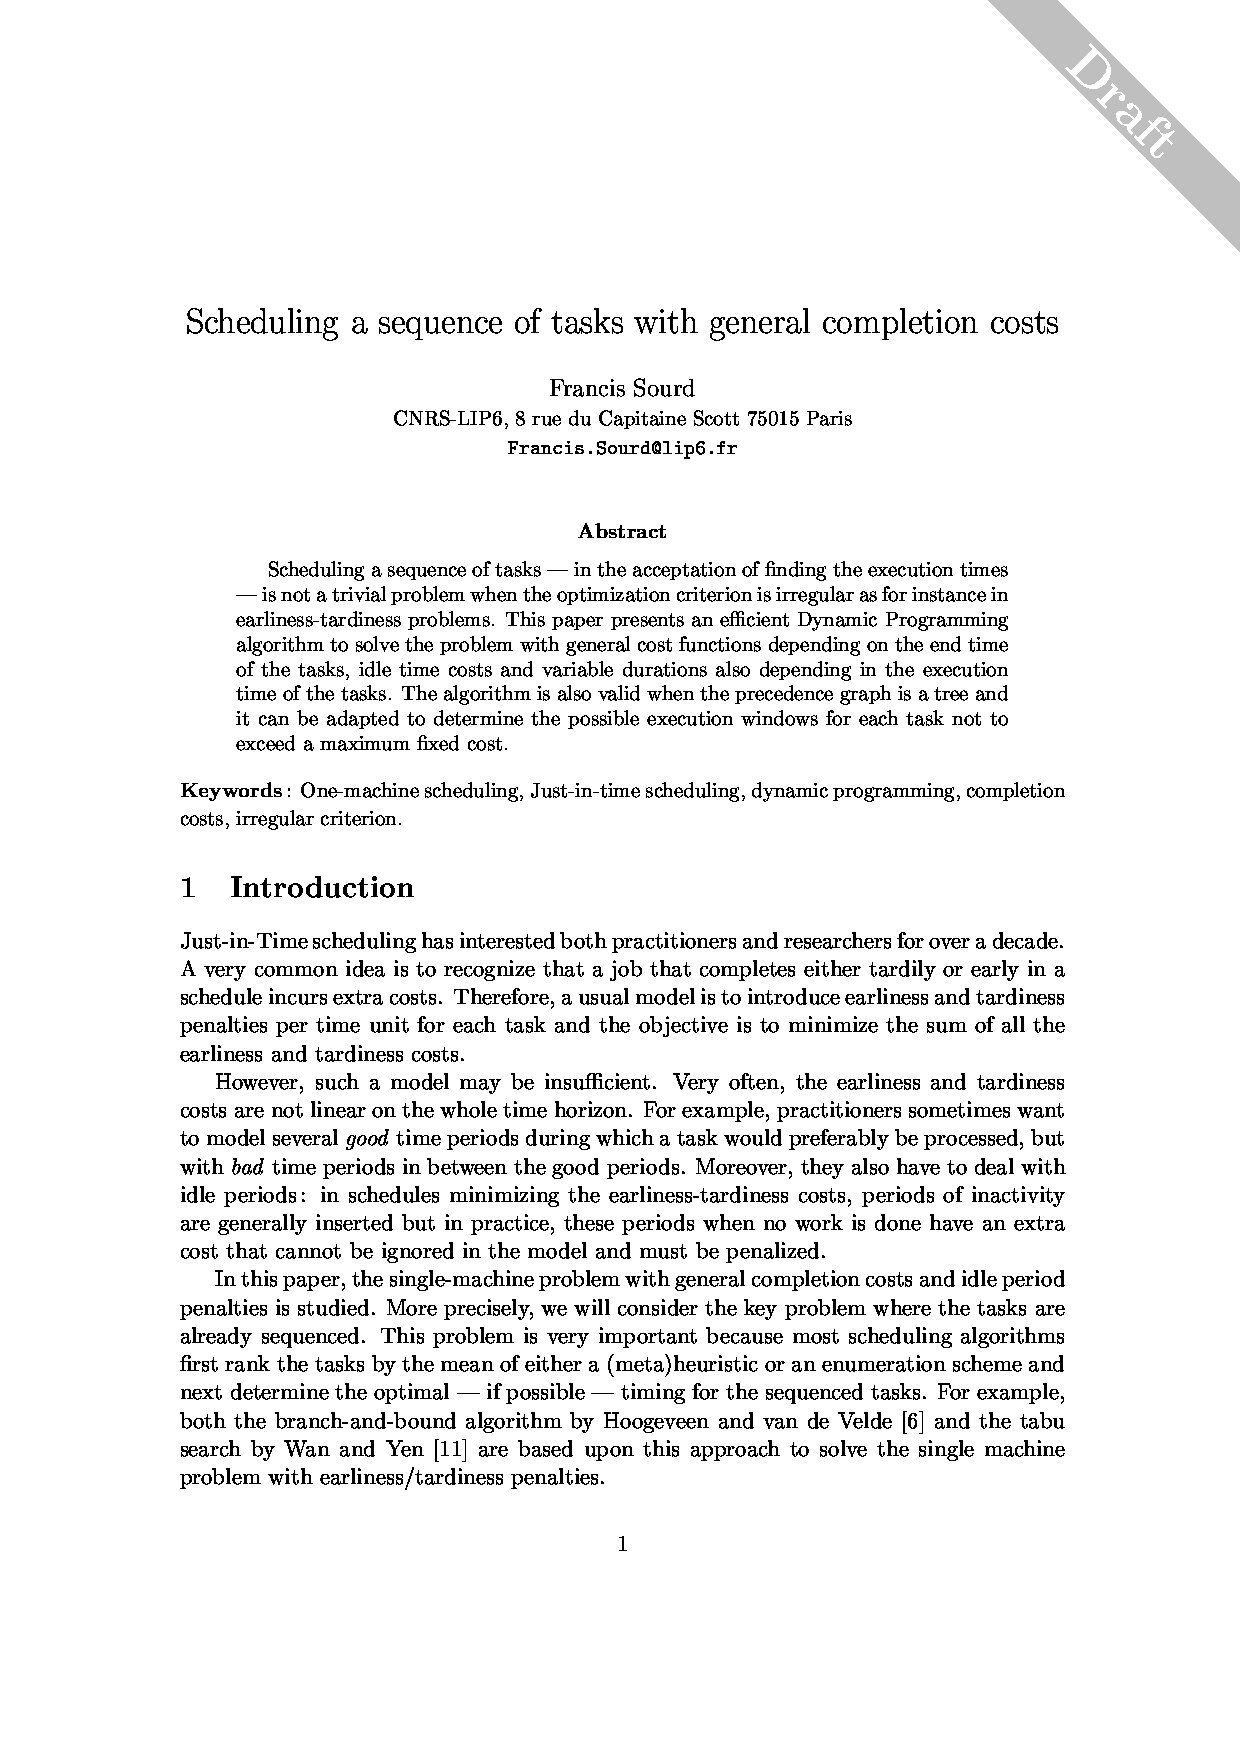
\includegraphics[width=6.5cm,keepaspectratio,clip]{sequence.pdf}
\caption{Example of sequence variable and no-overlap constraint}
\label{fig-sequence}
\end{figure}

\subsection{OPL Formulation}
\label{opl-sequence}

The construct below defines an interval sequence variable \verb|p| over a set of interval variables \verb|A| given as an array. The optional array of integers \verb|T| specifies the types of interval variables in the sequence, that is, \verb|T[i]| is the integer type of \verb|A[i]| in the sequence.

\begin{verbatim}
dvar sequence p in A [types T];
\end{verbatim}

Where 

\begin{verbatim}
dvar interval A[];
int T[];
\end{verbatim}

In OPL, the matrix used by the \verb|noOverlap| constraint needs to be defined as a set of integer triplets. Thus a matrix is a tuple set. For instance:

\begin{verbatim}
tuple triplet { int id1; int id2; int value; };  // 0<=id1, 0<=id2, 0<=value
{triplet} M = ...;
\end{verbatim}

The following constraints are available on interval sequence variables:

\begin{verbatim}
first (p, a);
last  (p, a);
prev  (p, a, b);
before(p, a, b);
\end{verbatim} 

\note{Important}{{\bf In the current version of \cp, the constraints {\tt first}, {\tt last}, {\tt prev} and {\tt before} cannot be used in meta-constraints.} }

The constraint(s) below define(s) how a given sequence of intervals influences the values of the interval themselves: 

\begin{verbatim}
noOverlap(p [,M]);
\end{verbatim} 

% TODO: also max transition distances

An additional construction of $\verb|noOverlap|$ is available that shortcuts the creation of the interval sequence variable for simple cases where the sequence is not useful:

\begin{verbatim}
noOverlap(A); // Same as: dvar sequence p in A; 
              //          noOverlap(p);
\end{verbatim}

\note{Important}{{\bf The constraint {\tt noOverlap} cannot be used in meta-constraints.}}

\subsection{Examples}

\begin{itemize}

\item A set of \verb|2*n| activities to be sequenced on a unary resource such that \verb|A[2*i-1]| is constrained to be executed immediately before to \verb|A[2*i]|.

\begin{verbatim}
dvar interval A[i in 1..2*n] size d[i];
dvar sequence p in A;

subject to {
  noOverlap(p);
  forall (i in 1..n)
    prev(p, A[2*i-1], A[2*i]);
}
\end{verbatim}

\item A set of \verb|n| activities \verb|A[i]| of integer type \verb|T[i]| to be sequences on a machine with a sequence dependent setup time \verb|abs(ti-tj)| to switch from activity type \verb|ti| to activity type \verb|tj|.

\begin{verbatim}
{int} Types = { T[i] | i in 1..n };
tuple triplet { int id1; int id2; int value; }; 
{triplet} M = { <i,j,ftoi(abs(i-j))> | i in Types, j in Types };

dvar interval A[i in 1..n] size d[i];
dvar sequence p in A types T;

subject to {
  noOverlap(p, M);
}
\end{verbatim}

\item Here is a complete model of an open-shop scheduling problem:

\begin{verbatim}
tuple Operation {
  int job; // Job
  int mch; // Machine
  int pt;  // Processing time
}

int NbJobs  = ...;
int NbMchs  = ...;
{Operation} Ops = ...;

dvar interval itvs[o in Ops] size o.pt;
dvar sequence jobs[j in 1..NbJobs] in all(o in Ops:o.job==j) itvs[o];
dvar sequence mchs[m in 1..NbMchs] in all(o in Ops:o.mch==m) itvs[o];

minimize max(o in Ops) endOf(itvs[o]);
subject to {
 forall(j in 1..NbJobs)
    noOverlap(jobs[j]);
 forall(m in 1..NbMchs)
    noOverlap(mchs[m]);
}
\end{verbatim}
\end{itemize}

\section{Cumul Functions} 
\label{cumul}

\subsection{Semantics}

\subsubsection{Informal Description}

In scheduling problems involving cumulative resources (also known as renewable resources), the cumulated usage of the resource by the activities is usually represented by a function of time. An activity usually increases the cumulated resource usage function at its start time and decrease it when it releases the resource at its end time (pulse function). For resources that can be produced and consumed by activities (for instance the content of an inventory or a tank), the resource level can also be described as a function of time, production activities will increase the resource level whereas consuming activities will decrease it. In these type of problems, the cumulated contribution of activities on the resource can be represented by a function of time and constraints can be posted on this function, for instance a maximal or a safety level.

\cp\ introduces the notion of {\em cumul function expression} which is a function that represents the sum of individual contributions of intervals. A panel of elementary cumul function expressions is available to describe the individual contribution of an interval variable (or a fixed interval of time), they cover the main use-cases mentioned above: {\em pulse} for usage of a cumulative resource, {\em step} for resource production/consumption (see \S\ref{cumul-func}). When the elementary cumul function expressions that define a cumul function expression are fixed (and thus, so are their related intervals), the expression is fixed. \cp\ provides several constraints over cumul function expressions. These constraints allow restricting the possible values of the function over the complete horizon or over some fixed or variable interval (see \S\ref{cumul-constraints}). For applications where the actual quantity of resource that is used, produced or consumed by intervals is an unknown of the problem, expressions are available for constraining these quantities (see \S\ref{cumul-intexprs}).

\subsubsection{Cumul Function Expressions}
\label{cumul-func}

Let $\cal{F}^+$ denote the set of all functions from $\Z$ to $\Z^+$. A {\bf cumul function expression} $f$ is an expression whose value is a function of $\cal{F}^+$ and thus, whose domain $dom(f)$ is a subset of $\cal{F}^+$. Let $u,v \in \Z$ and $h, h_{min}, h_{max} \in \Z^+$ and $a$ be an interval variable, we consider the following {\bf elementary cumul function expressions} illustrated in Figure \ref{fig:shapes}:
$pulse(u,v,h)$, 
$step(u,h)$, 
$pulse(a,h)$, 
$pulse(a,h_{min},h_{max})$, 
$stepAtStart(a,h)$, 
$stepAtStart(a,h_{min},h_{max})$,\linebreak
$stepAtEnd(a,h)$, 
$stepAtEnd(a,h_{min},h_{max})$.  

\begin{figure}[ht]
\centering
\includegraphics[width=9cm,keepaspectratio,clip]{shapes.pdf}
\caption{Elementary cumul function expressions}
\label{fig:shapes}
\end{figure}

More formally, let $u,v \in \Z$ and $h \in \Z^+$, we define the following particular functions of $\cal{F}^+$:
\begin{itemize}
\item $\underline{0}$ is the null function that is, the function $F$ such that $\forall t \in \Z, F(t)=0$
\item $\underline{pulse}(u,v,h)$ is the function $F$ such that $F(t)=h$ if $t \in [u,v)$, $F(t)=0$ otherwise
\item $\underline{step}(u,h)=\underline{pulse}(u,+\infty,h)$
\end{itemize}

The semantics of the elementary function expressions is listed on table \ref{tab:AtomicFunctions} together with the formal definition of their domain. The function set $0_a$ is equal to the singleton $\{ \underline{0} \}$ if $\bot \in dom(a)$, that is, if interval variable $a$ is possibly absent and equal to the empty set otherwise.

\begin{table}[htbp]
	\centering
		\begin{tabular}{|l|l|} \hline
		{\bf Function expression}  & {\bf Domain} \\ \hline \hline
		$pulse(u,v,h)$           & $\{\ \underline{pulse}(u,v,h)\ \}$ (singleton) \\ \hline
		$step(u,h)$              & $\{\ \underline{step}(u,h)\ \}$ (singleton) \\ \hline \hline
		$pulse(a,h)$             & $0_a \cup \{\ \underline{pulse}(s(\underline{a}),e(\underline{a}),h)\,|\,\underline{a}\in dom(a) \setminus \bot \ \}$ \\ \hline
		$pulse(a,h_{min},h_{max})$       & $0_a \cup \{\ \underline{pulse}(s(\underline{a}),e(\underline{a}),h)\,|\, h \in [h_{min},h_{max}] \land \underline{a}\in dom(a) \setminus \bot \ \}$ \\ \hline
		$stepAtStart(a,h)$       & $0_a \cup \{\ \underline{step}(s(\underline{a}),h)\,|\,\underline{a}\in dom(a) \setminus \bot \ \}$ \\ \hline
    $stepAtStart(a,h_{min},h_{max})$ & $0_a \cup \{\ \underline{step}(s(\underline{a}),h)\,|\,h \in [h_{min},h_{max}] \land \underline{a}\in dom(a) \setminus \bot \ \}$ \\ \hline
		$stepAtEnd(a,h)$         & $0_a \cup \{\ \underline{step}(e(\underline{a}),h)\,|\,\underline{a}\in dom(a) \setminus \bot \ \}$ \\ \hline
    $stepAtEnd(a,h_{min},h_{max})$   & $0_a \cup \{\ \underline{step}(e(\underline{a}),h)\,|\,h \in [h_{min},h_{max}] \land \underline{a}\in dom(a) \setminus \bot \ \}$ \\ \hline
    \end{tabular}
   \caption{Elementary cumul function expressions}
	\label{tab:AtomicFunctions}
\end{table}
    
A {\bf cumul function expression} $f$ is an expression built as the algebraical sum of the elementary function expressions of table \ref{tab:AtomicFunctions} or their negations. More formally, it is a construct of the form $f = \sum_i \epsilon_i \cdot f_i$ where $\epsilon_i \in \{-1,+1\}$ and $f_i$ is an elementary function expression. 

When all elementary function expressions $f_i$ related with a cumul function expression $f$ are fixed (that is, their domain is reduced to a singleton $\underline{f}_i$), the value of the cumul function expression $f$ is fixed and equal to the function $\underline{f} = \sum_i \epsilon_i \cdot \underline{f}_i$.
    
\subsubsection{Constraints on Cumul Function Expressions}
\label{cumul-constraints}

The following constraints can be expressed on a cumul function expression $f$. Let $u,v \in \Z$ and $h_{min}, h_{max} \in \Z^+$ and $a$ be an interval variable:

\begin{itemize}
\item $alwaysIn(f,u,v,h_{min},h_{max})$ means that the values of function $f$ must remain in the range $[h_{min},h_{max}]$ everywhere on the interval $[u,v)$.
\item $alwaysIn(f,a,h_{min},h_{max})$ means that if interval $a$ is present,
the values of function $f$ must remain in the range $[h_{min},h_{max}]$ between the start and the end of interval variable $a$.
\item $f \leq h_{max}$ means that function $f$ cannot take values greater than $h_{max}$. It is semantically equivalent to $alwaysIn(f,-\infty,+\infty,0,h_{max})$. 
\item $f \geq h_{min}$ means that function $f$ cannot take values lower than $h_{min}$. It is semantically equivalent to $alwaysIn(f,-\infty,+\infty,h_{min},+\infty)$. 
\end{itemize}

More formally:
\begin{eqnarray}
alwaysIn(\underline{f},u,v,h_{min},h_{max}) & \Leftrightarrow & \forall t \in [u,v),\ \underline{f}(t) \in [h_{min},h_{max}] \nonumber \\
alwaysIn(\underline{f},\underline{a},h_{min},h_{max}) & \Leftrightarrow & \forall t \in [s(\underline{a}),e(\underline{a})),\  \underline{f}(t) \in [h_{min},h_{max}] \nonumber
\end{eqnarray}

\subsubsection{Expressions on Cumul Function Expressions}
\label{cumul-intexprs}

The following elementary cumul function expressions are based on an interval variable $a$: 
$pulse(a,h)$, 
$pulse(a,h_{min},h_{max})$, 
$stepAtStart(a,h)$, 
$stepAtStart(a,h_{min},h_{max})$,
$stepAtEnd(a,h)$,\linebreak
$stepAtEnd(a,h_{min},h_{max})$.  

Some of these expressions define a range $[h_{min},h_{max}]$ of possible values for the actual height of the function when the interval variable $a$ is present. The actual height is an unknown of the problem. \cp\ provides some integer expressions to control this height. These expressions are based on the notion of contribution of a given interval variable $a$ to a (possibly composite) cumul function expression $f$. This contribution is defined as the sum of all the elementary cumul function expressions based on $a$ in $f$. This contribution is a discrete function that can change value only at the start and at the end of interval $a$ and is equal to $0$ before the start of $a$. 

For instance, let $a$ and $b$ be two interval variables and a cumul function expression $f$ defined by: $f = pulse(a,3) + pulse(a,2)- stepAtEnd(a,1) + stepAtStart(b,2) - stepAtEnd(b,3)$. The contribution of $a$ to $f$ is the function $pulse(a,3) + pulse(a,2)-stepAtEnd(a,1)$ and the contribution of $b$ to $f$ is the function $stepAtStart(b,2)-stepAtEnd(b,3)$.

If interval $a$ is present, the expression $heightAtStart(a, f)$ returns the value of the contribution of $a$ to $f$ evaluated at the start of $a$ that is, it measures the contribution of interval $a$ to cumul function expression $f$ at its start point. Similarly, the expression $heightAtEnd(a, f)$ returns the value of the contribution of $a$ to $f$ evaluated at the end of $a$ that is, it measures the contribution of interval $a$ to cumul function expression $f$ at its end point. An additional integer value $dval$ can be specified at the construction of the expression in which case, that will be the value returned by the expression when the interval is absent otherwise, if no value is specified, the expression will be equal to $0$ when the interval is absent.

In the example above, assuming both interval $a$ and $b$ to be present we would get: $heightAtStart(a, f)=5$, $heightAtEnd(a, f)=4$, $heightAtStart(b, f)=2$, $heightAtEnd(b, f)=-1$. Of course, in general when using ranges for the height of elementary cumul function expressions, the $heightAtStart/End$ expressions will not be fixed until all the heights have been fixed by the search.

More formally, if an elementary cumul function expression $f_i$ is based on an interval variable, we denote $ivar(f_i)$ this interval variable. Let $f$ be a cumul function expression defined as $f = \sum_i \epsilon_i \cdot f_i$ where $\epsilon_i \in \{-1,+1\}$ where $f_i$ are elementary cumul function expressions. The contribution of an interval variable $a$ to $f$ is defined as $f|_a = \sum_{i\,|\,ivar(f_i)=a} \epsilon_i \cdot f_i$ and the expressions $heightAtStart/End$ are defined as follows:

\begin{itemize}
\item $heightAtStart(\underline{a}, \underline{f},dval) = \left\{ \begin{array}{ll}
                                \underline{f}|_{\underline{a}}(s(\underline{a})) & \textrm{if $x(\underline{a})$}\\
                                dval & \textrm{otherwise}
                                \end{array} \right.$
\item $heightAtEnd(\underline{a}, \underline{f},dval) = \left\{ \begin{array}{ll}
                                \underline{f}|_{\underline{a}}(e(\underline{a})) & \textrm{if $x(\underline{a})$}\\
                                dval & \textrm{otherwise}
                                \end{array} \right.$                           
\end{itemize}

\subsection{OPL Formulation}

A type of expression \verb|cumulFunction| is introduced. The following functions build elementary cumul function expressions:

\begin{verbatim}
cumulFunction f = pulse(u,v, h);
cumulFunction f = pulse(a, h);
cumulFunction f = pulse(a, hmin, hmax);
cumulFunction f = step(u, h);
cumulFunction f = stepAtStart(a, h);
cumulFunction f = stepAtStart(a, hmin, hmax);
cumulFunction f = stepAtEnd(a, h);
cumulFunction f = stepAtEnd(a, hmin, hmax); 
\end{verbatim}

Where 
\begin{verbatim}
int u;
int v;
int h;
int hmin
int hmax;
int dval;
cumulFunction f;
cumulFunction g;
cumulFunction h;
cumulFunction F[];
cumulFunction G[];
dvar interval a; 
\end{verbatim}

A composite cumul function expression can be defined as a sum of cumul function expressions, it can be built using a \verb|sum| construct and possibly some \verb|-| operators, for instance: 

\begin{verbatim}
cumulFunction h = sum(i in ...) F[i] - sum(j in ...) G[j]; 
\end{verbatim}

The following are constraints on a cumul function expression \verb|f|:

\begin{verbatim}
f <= hmax;
hmin <= f;
alwaysIn(f, u, v , hmin, hmax);
alwaysIn(f, a, hmin, hmax);
\end{verbatim}

\note{Important}{{\bf All cumul function expressions {\tt f} involved in a {\tt <=} or an {\tt alwaysIn} constraint are constrained to be non-negative. Constraints {\tt <=} an {\tt alwaysIn} on cumul function expressions cannot be used in meta-constraints.} }

The following expressions are available on cumul function expressions:

\begin{verbatim}
dexpr int h = heightAtStart(a,f[,dval]);
dexpr int h = heightAtEnd(a,f[,dval]); 
\end{verbatim}

\subsection{Examples}

\begin{itemize}

\item A set of producing and consuming activities on a tank with a given capacity and safety level.

\begin{verbatim}
int Horizon     = ...;
int Capacity    = ...;
int SafetyLevel = ...;
int StartLevel  = ...;
int QProd[p in 1..NProd] ...;
int QCons[c in 1..NCons] ...;

dvar interval AProd[p in 1..NProd] ...;
dvar interval ACons[c in 1..NCons] ...;

cumulFunction level =
    step(0, StartLevel)
  + sum (p in 1..NProd) stepAtEnd(AProd[p], QProd[p])
  - sum (c in 1..NCons) stepAtStart(ACons[c], QCons[c]);
  
subject to {
  alwaysIn(level, 0, Horizon, SafetyLevel, Capacity);
}
\end{verbatim}

\item Here is a complete model of the classical Resource-Constrained Project Scheduling problem (with renewable resources only):

\begin{verbatim}
tuple Prec {
  int task1;
  int task2;
}

tuple Req {
  int task;
  int rsrc;
  int qtty;
}

int nbTasks = ...;
int nbRsrcs = ...;
int dur[i in 1..nbTasks] = ...;
int cap[j in 1..nbRsrcs] = ...;
{Prec} precs = ...;
{Req}  reqs  = ...;

dvar interval tasks[i in 1..nbTasks] size dur[i];
  
minimize max(i in 1..nbTasks) endOf(tasks[i]);
subject to {
 forall(p in precs)
   endBeforeStart(tasks[p.task1],tasks[p.task2]);
 forall(j in 1..nbRsrcs)
   sum (r in reqs: r.rsrc==j) pulse(tasks[r.task],r.qtty) <= cap[j];
}
\end{verbatim}

\item A set of $n$ activities $A_i$ of length $i$ and using $n-i$ units of a renewable resource have to be scheduled within a fixed horizon. The objective is to minimize the peak usage of the resource. A pulse with variable height is created for modelling the free amount of resource and the objective maximizes this free amount (height of the pulse). 

\begin{verbatim}
int n       = 100;
int horizon = 500;
int capMax  = 500;

dvar interval cover in 0..horizon size horizon;
dvar interval a[i in 1..n] in 0..horizon size i;
cumulFunction free  = pulse(cover, 0, capMax);
cumulFunction level = sum(i in 1..n) pulse(a[i],n-i) + free;
dexpr int peak = capMax - heightAtStart(cover, free);

minimize peak;
subject to {
  level <= capMax;
}
\end{verbatim}

\item A set of $n$ activities $A_i$ is defined. These activities may overlap (a set of constraints is defined on these activities but this is not the point of the code sample). This code sample defines $W$, a chain of at most $n$ intervals that exactly represent the set of time-windows during which at least one activity $A_i$ executes. The two {\tt alwaysIn} constraints state that (1) over each interval $W[i]$, there must be at least one activity executing ($1 \leq CA \leq n$) and (2) any date $t$ where an activity $A[i]$ executes must be covered by one (and exactly one) interval $W$ (thus, $CW==1$). These interval variables $W$ and cumul function expression $CW$ can be useful for instance to model a constraint stating that there cannot be more than a certain number of activities of a given type executing in parallel by computing one function $CW$ per type and constraining the sum of these functions. 

\begin{verbatim}
int horizon = ...;
int n = ...;
dvar interval A[i in 1..n] ...;
cumulFunction CA = sum(i in 1..n) pulse(A[i],1);
dvar interval W[i in 1..n] optional size 1..horizon; 
cumulFunction CW = sum(i in 1..n) pulse(W[i],1);
constraints {
  forall(i in 1..n-1) {
    endBeforeStart(W[i],W[i+1],1);
    presenceOf(W[i+1]) => presenceOf(W[i]);
  }
  forall(i in 1..n) {
    alwaysIn(CA, W[i], 1, n);
    alwaysIn(CW, A[i], 1, 1);
  }
  // Constraints on activities A[i] 
  // ...
}
\end{verbatim}

\end{itemize}

\section{State Functions} 
\label{state}

\subsection{Semantics}

\subsubsection{Informal Description}
\label{state-informal}

Some scheduling problems involve reasoning with resources whose state may change over time. The state of the resource can change because of the scheduled activities or because of exogenous events and some activities in the schedule may need a particular condition on the resource state to be true in order to execute. For instance, the temperature of an oven may change due to the execution of an activity that sets the oven temperature to a value $v$ and some cooking activity may require the oven temperature to be maintained at a temperature level $v'$ during its execution. In some applications, the transition between two states is not instantaneous and a transition time is needed for the resource to switch from a state $v$ to a state $v'$.

\cp\ introduces the notion of {\em state function} which is a function describing the evolution of a given feature of the environment. The possible evolution of this feature is constrained by interval variables of the problem. The main difference between state functions and cumul functions (see \S \ref{cumul}) is that interval variables have an incremental effect on cumul functions (increasing or decreasing the function value) whereas they have an absolute effect on state functions (requiring the function value to be equal to a particular state or in a set of possible states).

Informally speaking, a state function is a set of non-overlapping intervals over which the function maintains a particular non-negative integer state. In between those intervals, the state of the function is not defined, typically because of an ongoing transition between two states (see \ref{state-function}). For instance for an oven with 3 possible temperature levels identified by indexes $0$, $1$ and $2$ we could have: \\

\begin{tabular}{lll}
$[$start=0,   & end=100$)$: & state=0, \\
$[$start=150, & end=250$)$: & state=1,\\
$[$start=250, & end=300$)$: & state=1,\\
$[$start=320, & end=420$)$: & state=2,\\
$[$start=460, & end=560$)$: & state=0, $\cdots$ \\

\end{tabular}\\
 
A set of constraints are available to restrict the evolution of a state function (see \ref{state-constraints}). These constraints allows specifying:
\begin{itemize}
\item That the state of the function must be defined and should remain equal to a given non-negative state everywhere over a given fixed or variable interval ($alwaysEqual$).
\item That the state of the function must be defined and should remain constant (no matter its value) everywhere over a given fixed or variable interval ($alwaysConstant$).
\item That intervals requiring the state of the function to be defined cannot overlap a given fixed or variable interval ($alwaysNoState$).
\item That everywhere over a given fixed or variable interval, the state of the function, if defined, must remain within a given range of non-negative states $[v_{min},v_{max}]$ ($alwaysIn$).
\end{itemize}

Additionally, the constraints $alwaysEqual$ and $alwaysConstant$ can be complemented to specify that the given fixed or variable interval should have its start and/or end point synchronized with the start and/or end point of the interval of the state function that maintains the required state. This is the notion of {\em start} and {\em end alignment} which is particularly useful for modelling parallel batches. For instance in the oven example above, all interval variables that would require an oven temperature of level $1$ and specify a start and end alignment, if executed over the interval $[150,250)$ would have to start exactly at $150$ and end at $250$. This is depicted on figure \ref{fig:state} where $a_1$ and $a_2$ are two start and end aligned interval variables, $a_3$ is start aligned only and $a_4$ is not aligned at all.

\begin{figure}[ht]
\centering
\includegraphics[width=10cm,keepaspectratio,clip]{state.pdf}
\caption{State function and interval variable alignments}
\label{fig:state}
\end{figure}

\subsubsection{State Functions and Transition Distance}
\label{state-function}

A {\bf state function} $f$ is a decision variable whose value is a set of non-overlapping intervals, each interval $[s_i,e_i)$ being associated a non-negative integer value $v_i$ that represents the state of the function over the interval. 

Let  $\underline{f}$ be a fixed state function, we will denote $\underline{f}=(\ [s_i,e_i):v_i\ )_{i \in [1,n]}$:
\begin{itemize}
\item $\forall i \in [1,n], s_i \in \Z, e_i \in \Z, v_i \in \Z^+, s_i < e_i$
\item $\forall i \in [1,n-1], e_i \leq s_{i+1}$
\end{itemize}

We denote $D(\underline{f})= \cup_{i \in [1,n]}[s_i,e_i)$ the definition domain of $\underline{f}$, that is, the set of points where the state function is associated a state.

For a fixed state function $\underline{f}$ and a point $t \in D(\underline{f})$, we will denote $[s(\underline{f},t),e(\underline{f},t))$ the unique interval of the function that contains $t$ and $\underline{f}(t)$ the value of this interval:

\[ [s(\underline{f},t),e(\underline{f},t)) = [s_i, e_i), t \in [s_i, e_i) \]
\[ \underline{f}(t) = v_i, t \in [s_i, e_i) \]

For instance, in the example of the oven introduced in section \ref{state-informal}, we would have $\underline{f}(200)=1$, $s(\underline{f},200)=150$ and $e(f,200)=250$.

A state function can be associated a {\bf transition distance}. The transition distance defines the minimal distance that must separate two consecutive states in the state function. 

More formally, if $M[v,v']$ represent a transition distance matrix between state $v$ and state $v'$, the transition distance means that: 

\[\forall i \in [1,n-1], e_i + M[v_i,v_{i+1}] \leq s_{i+1}\]

The transition distance matrix $M$ must satisfy the triangular inequality.

For instance, in the example of the oven, the state function depicted on Figure \ref{fig:state} is consistent with the following transition distance:
\begin{displaymath}
\mathbf{M} =
\left( \begin{array}{ccc}
0 & 50 & 60 \\
20 & 0 & 20 \\
40 & 30 & 10
\end{array} \right)
\end{displaymath}
Notice that a transition distance between the same states can be non-zero, as
it is for state $3$ in this example.

\subsubsection{Constraints on State Functions}
\label{state-constraints}

If $f$ is a state function, $a$ an interval variable, $v$, $v_{min}$, $v_{max}$ non-negative integers and $algn_s$, $algn_e$ two boolean values:
\begin{itemize}
\item The constraint $alwaysEqual(f,a,v,algn_s,algn_e)$ specifies that whenever interval variable $a$ is present, $a$ must be contained in an interval where state function $f$ maintains non-negative state $v$. If $salgn$ is true, it means that interval $a$ is start-aligned with $f$: interval $a$ must start at the beginning of the interval where $f$ is maintained in state $s$. If $ealgn$ is true, it means that interval $a$ is end-aligned with $f$: interval $a$ must end at the end of the interval where $f$ is maintained in state $s$. More formally:
  \begin{enumerate}[(a)]
  \item[(a)] $[s(\underline{a}),e(\underline{a})) \subset [s(\underline{f},s(\underline{a})), e(\underline{f},s(\underline{a})))$
  %\item $\forall t \in [s(\underline{a}),e(\underline{a})), t \in D(\underline{f}) \land \underline{f}(t)=v$
  \item[(b)] $algn_s \Rightarrow s(\underline{a})=s(\underline{f},s(\underline{a}))$
  \item[(c)] $algn_e \Rightarrow e(\underline{a})=e(\underline{f},e(\underline{a}))$ 
  \end{enumerate}
\item The constraint $alwaysConstant(f,a,algn_s,algn_e)$ specifies that whenever $a$ is present, state function $f$ must be defined everywhere between the start and the end of interval $a$ and be constant over this interval. More formally: $\exists v \in Z^+, alwaysEqual(f,a,v,algn_s,algn_e)$
\item The constraint $alwaysNoState(f,a)$ specifies that whenever $a$ is present, state function $f$ cannot provide any valid state between the start and the end of interval $a$. As a consequence, any interval constrained with $alwaysEqual$ or $alwaysConstant$ on this function and thus requiring the function to be defined cannot overlap interval $a$. More formally, the constraint means that $[s(\underline{a}),e(\underline{a})) \cap D(\underline{f})=\emptyset$.
\item The constraint $alwaysIn(f,a,v_{min},v_{max})$ where $0 \leq v_{min} \leq v_{max}$ specifies that whenever $a$ is present, everywhere between the start and the end of interval $a$ the state of function $f$, if defined, must belong to the range $[v_{min},v_{max}]$. Formally: $\forall t \in [s(\underline{a}),e(\underline{a})) \cap D(\underline{f}), \underline{f}(t) \in [v_{min},v_{max}]$.
\end{itemize}

On Figure \ref{fig:state}, there are two adjacent intervals of state $1$: the first one
is $[150, 250)$ and the second one $[250, 300)$. There are two reasons for
that: $250$ is end of end-aligned interval $a_1$ and also start of
start-aligned interval $a_2$. Therefore due to condition (b) or (c) the
interval $[150,300)$ must be split in two (even though the state function
does not change its value). Note also that thanks to condition (a) the
interval $a_4$ cannot overlap $250$, despite the fact that $a_4$ is neither
start nor end aligned. To allow $a_4$ overlap $250$ it would be necessary to
use $alwaysIn$ constraint instead of $alwaysEqual$ -- the difference is that
$alwaysIn$ does not enforce condition (a) even if the allowed state range is
singleton (however, $alwaysIn$ also allows the interval to overlap with
state transitions).


\subsection{OPL Formulation}

A type \verb|stateFunction| is introduced. The following statement builds a state function:

\begin{verbatim}
stateFunction f [with M];
\end{verbatim}

Where the optional argument \verb|M| is a transition matrix that needs to be defined as a set of integer triplets (just like for the \verb|noOverlap| constraint, see \ref{opl-sequence}). Thus this matrix is a tuple set. For instance:

\begin{verbatim}
tuple triplet { int v1; int v2; int dist; }; 
{ triplet } M = ...;
\end{verbatim}

The following are constraints over a state function \verb|f|:

\begin{verbatim}
alwaysEqual    (f,s,e,v[,aligns,aligne]);
alwaysEqual    (f,a,v[,aligns,aligne]); 
alwaysConstant (f,s,e [,aligns,aligne]);
alwaysConstant (f,a[,aligns,aligne]);
alwaysNoState  (f,s,e);
alwaysNoState  (f,a);
alwaysIn       (f,s,e,vmin,vmax);
alwaysIn       (f,a,vmin,vmax);
\end{verbatim}

Where 
\begin{verbatim}
int s; 
int e;            // s <= e
int v;            // 0 <= v
int vmin;         // 0 <= vmin
int vmax;         // vmin <= vmax
dvar interval a;
bool aligns;
bool aligne;
\end{verbatim}

\note{Important}{{\bf Constraints {\tt alwaysEqual}, {\tt alwaysConstant}, {\tt alwaysNoState} and {\tt alwaysIn} on state functions cannot be used in meta-constraints.} }

\subsection{Examples}


\begin{itemize}

%% MACHINE WITH TOOLS
\item A machine can be equipped with a tool among a set of $n$ possible tools. Each operation $o$ executed on the machine needs a specific tool $RequiredTool[o]$. The machine can process several operation simultaneously provided these operations are compatible with the tool currently installed on the machine. Changing the tool installed on the machine needs some constant set-up time which is supposed to be independent from the tools. 

\begin{verbatim}
int nbTools   = ...;
int nbOps     = ...;
int setupTime = ...;
range Tools      = 1..nbTools;
range Operations = 1..nbOps;
int Duration     [Operations] = ...;
int RequiredTool [Operations] = ...;
 
dvar interval op[o in Operations] size Duration[o];

tuple triplet { int tl1; int tl2; int value; }; 
{triplet} Transition = { <tl1,tl2,setupTime> | tl1, tl2 in Tools };
stateFunction machineTool with Transition;

constraints {
  forall(o in Operations) { 
     alwaysEqual(machineTool, op[o], RequiredTool[o]);
  }
}
\end{verbatim}

%% OVEN
\item A limited capacity oven is used to treat items in parallel batches.  Items requiring incompatible temperatures cannot be treated in the same batch. Some set-up time is needed to warm-up and cool-down the oven depending on the original and target temperature levels. The oven temperature is modelled as a state function. In a solution, the intervals of the state function represent the different batches. The treatment of each item is modelled by an interval variable. Because of parallel batching, items treated in the same batch need to be synchronized: they have the same start and end time, this is modelled using the notion of start and end alignment.

\begin{verbatim}
int MaxItemsInOven = ...;
int NbItems = ...;
range Items = 1..NbItems;
int DurationMin[Items] = ...;
int DurationMax[Items] = ...;
int Temperature[Items] = ...;
tuple triplet { int t1; int t2; int value; }; 
{triplet} Transition = ...;

dvar interval treat[i in Items] size DurationMin[i]..DurationMax[i];

stateFunction ovenTemperature with Transition;
cumulFunction itemsInOven = sum(i in Items) pulse(treat[i], 1);

constraints {
  itemsInOven <= MaxItemsInOven;
  forall(i in Items)
    alwaysEqual(ovenTemperature, treat[i], Temperature[i], 1, 1);
}
\end{verbatim}

Now suppose that a maintenance task is to be performed on the oven and that, during this maintenance task, the oven temperature should not reach high values (say, greater than level $4$). This could be modelled by the additional constraint:

\begin{verbatim}
dvar interval maintenance ...;

constraints {
  // ...
  alwaysIn(ovenTemperature, maintenance, 0, 4);
}
\end{verbatim}

\end{itemize}

\section{ILOG Script for OPL}

\subsection{CP Parameters for scheduling}

The following parameters are available to control the inference level in the \cp\ engine. As for other inference level parameters, their possible values are \verb|Low|, \verb|Basic|,  \verb|Medium| and \verb|Extended|.
The global default value in CP Optimizer is \verb|Basic|.

\begin{itemize}
\item \verb|PrecedenceInferenceLevel| controls the inference level of precedence constraints (See \S{\ref{temporal}})
\item \verb|IntervalSequenceInferenceLevel| controls the internal inference level of sequence variables (See \S{\ref{sequence-variables}})
\item \verb|NoOverlapInferenceLevel| controls the inference level of no-overlap constraints (See \S{\ref{no-overlap}})
\item \verb|CumulFunctionInferenceLevel| controls the inference level of constraints defined on cumul function expressions (See \S{\ref{cumul}})
\item \verb|StateFunctionInferenceLevel| controls the inference level of constraints defined on state functions (See \S{\ref{state}})
\item \verb|TemporalRelaxation| controls the usage of a temporal relaxation internal to engine. This parameter can take values "On" or "Off", with "On" being the default, meaning the relaxation is used in the engine when needed. For some models, using the relaxation becomes inefficient, and you may deactivate the use of the temporal relaxation using value "Off". This is an {\bf advanced} parameter.
\end{itemize}

\subsection{CP Search Phases for scheduling}

Two types of search phases are available for scheduling: search phases on interval variables and search phases on sequence variables. 

\begin{itemize}

\item A search phase on interval variables works on a unique interval variable or on an array of interval variables.  During this phase \cp\ fixes the value of the specified interval variable(s): each interval variable will be assigned a presence status and for each present interval, a start and an end value.
   
This search phase fixes the start and end values of interval variables in an unidirectional manner, starting to fix first the intervals that will be assigned a small start or end value.

\begin{verbatim}
searchPhase(a);
searchPhase(A);
\end{verbatim}

Where 
\begin{verbatim}
dvar interval a;
dvar interval A[];
\end{verbatim}

For instance, this code sample will specify a search that first fixes all interval variables in array \verb|A1| before the ones in array \verb|A2|.

\begin{verbatim}
dvar interval A1[...] ...;
dvar interval A2[...] ...;

execute {
  var f = cp.factory;
  cp.setSearchPhases(f.searchPhase(A1),
                     f.searchPhase(A2)); 
}
\end{verbatim}

\item A search phase on sequence variables works on a unique sequence variable or on an array of sequence variables.  During this phase \cp\ fixes the value of the specified sequence variable(s):  each sequence variable will be assigned a totally ordered sequence of present interval variables. Note that this search phase also fixes the presence statuses of the intervals involved in the sequence variables. This phase does not fix the start and end values of interval variables.
 
It is recommended to use this search phase only if the possible range for start and end values of all interval variables is limited (for example by some known horizon that limits their maximal values).  

\begin{verbatim}
searchPhase(p);
searchPhase(P);
\end{verbatim}

Where 
\begin{verbatim}
dvar sequence p;
dvar sequence P[];
\end{verbatim}

\end{itemize}


\subsection{Accessing solutions in postprocessing }

The value of an interval variable \verb|a| in a solution can be accessed using the following instructions:
\begin{itemize}
\item \verb|a.present| returns a boolean describing whether or not interval \verb|a| is present in the solution.
\item for a present interval, \verb|a.start|, \verb|a.end| and \verb|a.size| respectively return the start, end and size value of interval \verb|a| in the solution.
\end{itemize}

For instance the following postprocessing code will display the values of a set of interval variables in a solution.

\begin{verbatim}
dvar interval a[i in 1..n] ...;

// Model
// ...

// Postprocessing
execute {
 for(var i=1; i<=n; i++) {
    if (a[i].present) {
      writeln("Activity ", i, " executed on [", a[i].start, ",", a[i].end, ")");
    } else {
      writeln("Activity ", i, " is not executed");
    }
  }
}
\end{verbatim}

An interval variable \verb|a| in a solution can be displayed using \verb|writeln(a)|. This instruction displays a vector: \verb|< a.present a.start a.end a.size >|.

The value of a sequence variable \verb|p| in a solution can be accessed using the following instructions:
\begin{itemize}
\item \verb|p.first()| and \verb|p.last()| respectively return the interval variable that corresponds to the first (resp. last) interval of the sequence. In case the sequence is empty the returned value is \verb|null|.  
\item \verb|p.next(a)| and \verb|p.prev(a)| respectively return the interval variable sequenced just after \verb|a| (resp. just before \verb|a|) in the sequence. In case \verb|a| is the last (resp. first) interval in the sequence, the returned value is \verb|null|. 
\end{itemize}

For instance, the following postprocessing code displays in chronological order the start end end dates of the intervals in a sequence variable.

\begin{verbatim}
dvar interval a[i in 1..n] size i;
dvar sequence s in all(i in 1..n) a[i];

// Model
// ...

// Postprocessing
execute {
  for(var x=s.first(); x!=null; x=s.next(x)) {
    writeln("[", x.start, ",", x.end, ")");
  }
}
\end{verbatim}

A sequence variable \verb|p| in a solution can be displayed using \verb|writeln(p)|. This instruction displays the set of present interval variables in the sequence following the total order specified by the sequence.

In a solution, a cumul function \verb|f| is a non-negative step function. The value of a cumul function \verb|f| in a solution can be accessed using the following instructions:
\begin{itemize}
\item \verb|numberOfSegments(f)| returns an integer value that corresponds to the number of segments of cumul function \verb|f| in the solution.
\item \verb|segmentStart(f,i)| returns the start of the $i^{th}$ segment of cumul function \verb|f| in the solution.
\item \verb|segmentEnd(f,i)| returns the end of the $i^{th}$ segment of cumul function \verb|f| in the solution.
\item \verb|segmentValue(f,i)| returns the value of the $i^{th}$ segment of cumul function \verb|f| in the solution.
\item \verb|cumulFunctionValue(f,t)| returns the value of cumul function \verb|f| at point \verb|t| in the solution.
\end{itemize}

For instance, the following postprocessing code displays the steps of a cumul function in a solution. 

\begin{verbatim}
dvar interval a[i in 1..n] size i;
cumulFunction f = sum(i in 1..n) pulse(a[i],i); 

// Model
// ...

// Postprocessing
execute {
  for(var i=0; i<Opl.numberOfSegments(f); i++) {
    writeln("Step[", i, "]: value=", Opl.segmentValue(f,i), 
            " on [", Opl.segmentStart(f,i), "," , Opl.segmentEnd(f,i), ")");
  }
}
\end{verbatim}

\appendix
\newpage

\section{Notations}
\label{notations}

The main notations are summarized on Table \ref{tab:MainNotations}. Vectors are denoted by capital letters, for instance $Y$. The size of a vector $Y$ is denoted $|Y|$. If $n=|Y|$, the vector is denoted $Y=(y_1,...,y_n)$.

\begin{table}[h]
	\centering
		\begin{tabular}{|l|l|l|} \hline
		{\bf Notation}          & {\bf Type}           & {\bf Description}  \\ \hline \hline
    $a$, $b$ 	              & interval variable	&  \\ \hline
    $x(a)$ 	                & boolean expression 	 & presence status of $a$ \\ \hline
    $s(a)$, $e(a)$, $l(a)$ 	& integer expression 	 & start, end, length of $a$ \\ \hline
    $sz(a)$ 	              & integer expression 	 & size of $a$ \\ \hline
    $A$, $B$ 	              & vector of interval variables &  \\ \hline 
    $p$                     & interval sequence variable	& \\ \hline
    $f, g, h$               & cumul function expression & \\ 
                            & state function            & \\ \hline \hline
    $\underline{a}$, $\underline{b}$ 	             & {\bf fixed} interval	& \\ \hline
    $x(\underline{a})$ 	    & boolean 	           & presence status of $\underline{a}$ \\ \hline
    $s(\underline{a})$, $e(\underline{a})$, $l(\underline{a})$ 	& integer  & start, end, length of $\underline{a}$ \\ \hline
    $sz(\underline{a})$ 	  & integer 	           & size of $\underline{a}$ \\ \hline
		$\pi$                   & interval variable permutation	&  \\ \hline
    $z$ 	                  & integer (expression) & delay of a precedence \\ \hline
    $t$ 	                  & integer 	           & date \\ \hline
    $T$                     & vector of integers   & array of dates \\ \hline
    $S$                     & vector of floats     & array of slopes \\ \hline
    $v,w$                   & integer or float     & miscellaneous integer or float value \\ \hline
    $V,W$                   & vector of integers or floats & vector of miscellaneous values \\ \hline
    $align$                 & boolean              & alignment flag \\ \hline
    $F$,$G$,$H$ 	          & piecewise linear function $\R \rightarrow \R$ 	&  \\
      	                    & vector of cumul function expressions &  \\ \hline
    $T(p,a)$                & integer   & type of interval $a$ in sequence $p$ \\ \hline
    $M$ 	                  & integer matrix 	     & transition distance matrix \\ \hline
    $\cal{F}^+$             & set of functions     & set of all functions $f: \Z \rightarrow \Z^+$ \\ \hline
 		\end{tabular}
	\caption{Main notations}
	\label{tab:MainNotations}
\end{table}


\bibliography{biblio}
% Length: 1.5 page

\bibliographystyle{plain}

\end{document}

